\section{Results}
\label{sec:results}

Table~\ref{tab:main} summarises the study; Figure~\ref{fig:support} plots
selection quality and active-set size against $E$; the complete grid is in
Table~\ref{tab:full}. All entries are means over $100$ replicates per
design, with Monte Carlo standard errors.

\begin{table}[t]
\centering
\small
\caption{Monte Carlo results over 100 replicates per design ($p=600$, $s=30$, $K=3$, $m=(400,240,160)$). Support metrics are against the true support at $\epsilon=10^{-4}$. Monte Carlo standard errors for $F_1$ in parentheses. \textsc{FedAvg} and \textsc{FedAvg-ST} are shown at $E=1$ and $E=20$; the full grid is in Table~\ref{tab:full}.}
\label{tab:main}
\begin{tabular}{llrrrrrrr}
\toprule
Design & Method & Active & Prec. & Recall & $F_1$ & $\|\hat\beta-\beta^\star\|_2$ & Test MSE & Rounds \\
\midrule
Independent & Pooled & 127.6 & 0.246 & 0.977 & 0.388 (0.008) & 1.94 & 24.43 & --- \\
 & Local-only & 105.5 & 0.260 & 0.863 & 0.395 (0.007) & 2.85 & 28.81 & 0.0 \\
 & One-shot & 198.4 & 0.150 & 0.940 & 0.257 (0.006) & 2.91 & 29.18 & 1.0 \\
 & ADMM & 43.6 & 0.681 & 0.875 & 0.738 (0.011) & 2.51 & 27.19 & 58.7 \\
 & FedAvg ($E=1$) & 253.6 & 0.125 & 0.955 & 0.218 (0.006) & 2.85 & 28.82 & 14.6 \\
 & FedAvg ($E=20$) & 203.1 & 0.149 & 0.940 & 0.255 (0.006) & 2.91 & 29.17 & 3.6 \\
 & FedAvg-ST ($E=1$) & 45.4 & 0.576 & 0.801 & 0.654 (0.009) & 3.21 & 31.03 & 15.6 \\
 & FedAvg-ST ($E=20$) & 46.0 & 0.565 & 0.795 & 0.644 (0.009) & 3.27 & 31.41 & 4.6 \\
\midrule
Correlated & Pooled & 121.1 & 0.255 & 0.968 & 0.399 (0.008) & 2.09 & 24.61 & --- \\
 & Local-only & 107.7 & 0.252 & 0.846 & 0.383 (0.007) & 3.03 & 28.91 & 0.0 \\
 & One-shot & 198.8 & 0.146 & 0.930 & 0.251 (0.005) & 3.04 & 28.83 & 1.0 \\
 & ADMM & 48.3 & 0.601 & 0.860 & 0.681 (0.011) & 2.58 & 27.15 & 93.8 \\
 & FedAvg ($E=1$) & 263.2 & 0.117 & 0.949 & 0.206 (0.005) & 2.96 & 28.42 & 16.5 \\
 & FedAvg ($E=20$) & 201.6 & 0.145 & 0.930 & 0.250 (0.005) & 3.03 & 28.83 & 3.8 \\
 & FedAvg-ST ($E=1$) & 59.3 & 0.457 & 0.805 & 0.565 (0.010) & 3.22 & 30.70 & 17.5 \\
 & FedAvg-ST ($E=20$) & 61.4 & 0.428 & 0.796 & 0.543 (0.010) & 3.29 & 31.08 & 4.8 \\
\midrule
Heterogeneous & Pooled & 116.1 & 0.256 & 0.888 & 0.388 (0.009) & 2.77 & 38.55 & --- \\
 & Local-only & 105.5 & 0.260 & 0.863 & 0.395 (0.007) & 2.85 & 39.23 & 0.0 \\
 & One-shot & 185.3 & 0.157 & 0.922 & 0.266 (0.005) & 3.10 & 40.25 & 1.0 \\
 & ADMM & 44.0 & 0.603 & 0.646 & 0.537 (0.014) & 3.33 & 42.28 & 66.1 \\
 & FedAvg ($E=1$) & 258.5 & 0.121 & 0.943 & 0.212 (0.005) & 3.05 & 40.05 & 14.2 \\
 & FedAvg ($E=20$) & 194.0 & 0.154 & 0.923 & 0.262 (0.006) & 3.10 & 40.24 & 4.0 \\
 & FedAvg-ST ($E=1$) & 23.5 & 0.830 & 0.593 & 0.654 (0.016) & 3.72 & 44.93 & 15.2 \\
 & FedAvg-ST ($E=20$) & 25.4 & 0.807 & 0.605 & 0.652 (0.013) & 3.75 & 45.14 & 5.0 \\

\bottomrule
\end{tabular}
\end{table}

\begin{figure}[t]
\centering
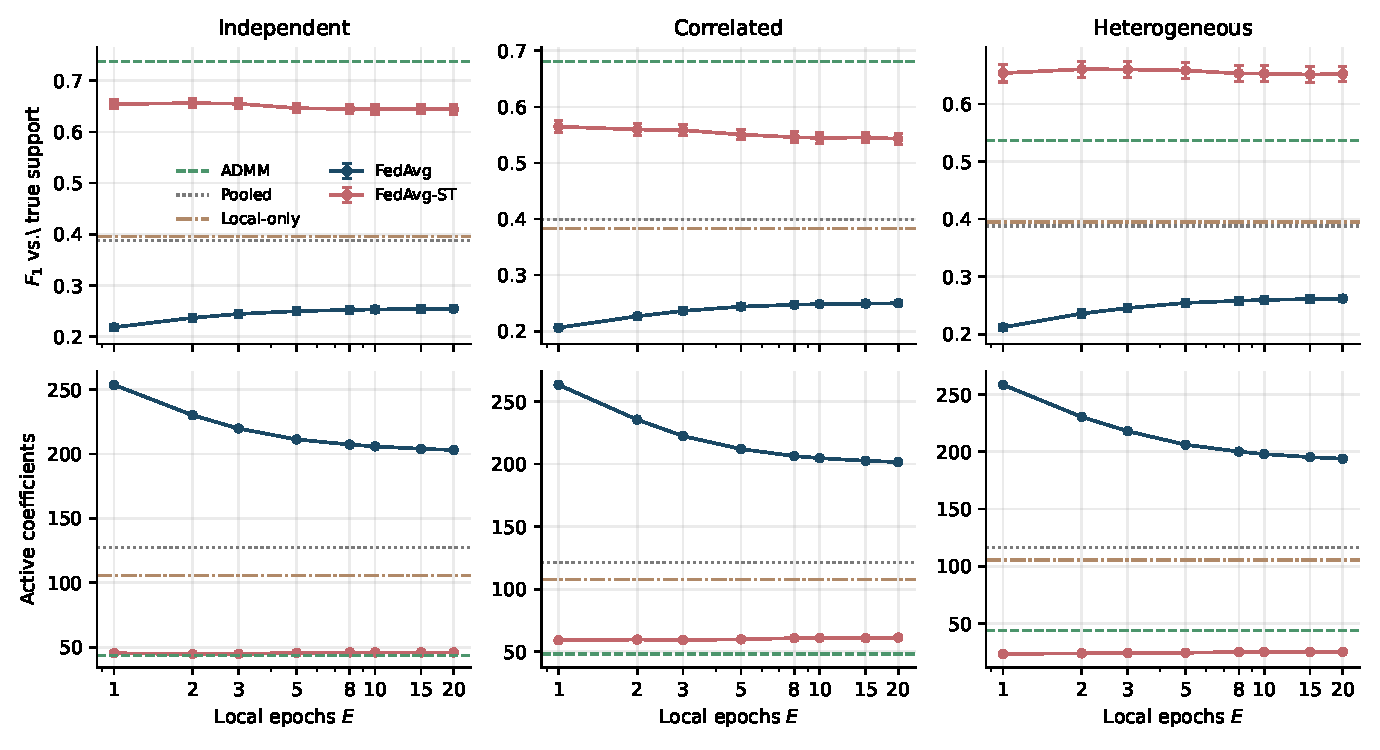
\includegraphics[width=\textwidth]{figures/fig1_support.pdf}
\caption{Selection quality (top) and active-set size (bottom) against the
number of local epochs $E$, by design. Error bars are Monte Carlo standard
errors over $100$ replicates. Horizontal lines are the comparators, which
do not depend on $E$. The true model has $s = 30$ non-zero coefficients out
of $p = 600$.}
\label{fig:support}
\end{figure}

\subsection{Plain averaging returns a dense estimator at every $E$}

The first row of Figure~\ref{fig:support} is dominated by a gap that has
nothing to do with $E$. With $s = 30$ true signals out of $p = 600$,
\textsc{FedAvg} declares \MIndFedActOne, \MCorFedActOne\ and
\MHetFedActOne\ coefficients active at $E = 1$ in the independent,
correlated and heterogeneous designs---between a third and a half of all
predictors. The signature is exactly the one predicted by
Proposition~\ref{prop:orth}(iv): recall is very high
(\MIndFedRecOne, \MCorFedRecOne, \MHetFedRecOne) and precision very low
(\MIndFedPrecOne, \MCorFedPrecOne, \MHetFedPrecOne). The aggregated
estimator misses almost no true signal and admits almost everything else,
which is what taking a union of three local active sets does.

Increasing $E$ shrinks the active set---by \MIndActDrop, \MCorActDrop\ and
\MHetActDrop\ from $E = 1$ to $E = 20$---and correspondingly raises $F_1$
from \MIndFedFOne\ to \MIndFedFTwenty, \MCorFedFOne\ to \MCorFedFTwenty,
and \MHetFedFOne\ to \MHetFedFTwenty. It would be natural to read this as
more local work producing better selection. The reading we prefer is that
more local work produces \emph{less union}: each site's iterate is closer
to its own sparse local minimiser, so fewer distinct coordinates survive
the average. Consistently with Proposition~\ref{prop:orth}(ii), the
shrinkage is smallest in the independent design and largest in the
heterogeneous one, though the ordering is modest and we would not want to
lean on it: with $p > m_j$ no design here is close to the orthogonal case
in which the $E$-effect is exactly zero.

Whatever the mechanism, the practical conclusion is the same at both ends
of the range: at every $E$ and in every design, plain averaging is far worse
at recovering the true support than \emph{doing nothing}. Fitting the Lasso
at the largest site alone gives $F_1 = \MIndLocF$, \MCorLocF\ and
\MHetLocF, against at most \MIndFedFTwenty, \MCorFedFTwenty\ and
\MHetFedFTwenty\ for \textsc{FedAvg}. Nor does the communication buy much:
by $E = 20$, \textsc{FedAvg} has converged to essentially the one-shot
average, which uses a single round
($F_1 = \MIndOneShotF$, \MCorOneShotF, \MHetOneShotF\ against
\MIndFedFTwenty, \MCorFedFTwenty, \MHetFedFTwenty).

\subsection{A server-side threshold recovers most of what averaging loses}

\textsc{FedAvg-ST} changes the picture substantially for one extra round of
scalar traffic. Active-set sizes fall to \MIndStActOne, \MCorStActOne\ and
\MHetStActOne, and $F_1$ rises to \MIndStFOne\ (SE \MIndStSeOne),
\MCorStFOne\ (\MCorStSeOne) and \MHetStFOne\ (\MHetStSeOne)---roughly
three times the plain-averaging value in the independent and heterogeneous
designs, and comfortably above both the local-only baseline and the pooled
Lasso, whose prediction-tuned penalty leaves it dense
(\MIndPoolAct, \MCorPoolAct, \MHetPoolAct\ active; $F_1 = \MIndPoolF$,
\MCorPoolF, \MHetPoolF). Like plain averaging, \textsc{FedAvg-ST} is
essentially flat in $E$, which is the point: once the aggregation rule is
repaired, the choice of $E$ is a communication-versus-computation decision
and no longer a variable-selection decision.

The improvement is not free, and the direction of the trade is worth
stating. Thresholding removes small non-zero coefficients that were
contributing to fit, so estimation and prediction deteriorate slightly:
in the independent design $\|\hat\bbeta - \bbeta^\star\|_2$ rises from
\MIndFedErrOne\ to \MIndStErrOne\ and test MSE from \MIndFedMseOne\ to
\MIndStMseOne. An analyst who wants a variable list should take that trade;
one who wants a predictor should not.

\subsection{Exact consensus dominates, except under heterogeneity}

Consensus ADMM, which minimises the same objective $F$ exactly, gives
$F_1 = \MIndAdmmF$ and \MCorAdmmF\ in the independent and correlated
designs with \MIndAdmmAct\ and \MCorAdmmAct\ active coefficients---the best
support recovery of any method considered, and by a wide margin over
anything based on averaging. This is the cleanest possible statement of the
article's point: holding the data, the objective, the penalty and the
privacy boundary fixed, and changing only how the sites are combined, $F_1$
moves from \MIndFedFOne\ to \MIndAdmmF.

The exception is instructive. In the heterogeneous design ADMM attains
$F_1 = \MHetAdmmF$, below \textsc{FedAvg-ST}'s \MHetStFOne. Exactness is a
property of the optimisation, not of the estimand: ADMM solves the pooled
Lasso at the weighted-average penalty $\bar\lambda$, and when sites differ
in design scale and noise level, $\bar\lambda$ is simply not a good common
penalty. \textsc{FedAvg-ST}, which selects its threshold on validation data,
adapts where ADMM cannot. Exact consensus also costs the most
communication: it needed \MIndAdmmRounds, \MCorAdmmRounds\ and
\MHetAdmmRounds\ rounds on average, against $\MIndRoundsOne$, $\MCorRoundsOne$ and
$\MHetRoundsOne$ for \textsc{FedAvg} at $E = 1$.

\subsection{Communication and computation move in opposite directions}

\begin{figure}[t]
\centering
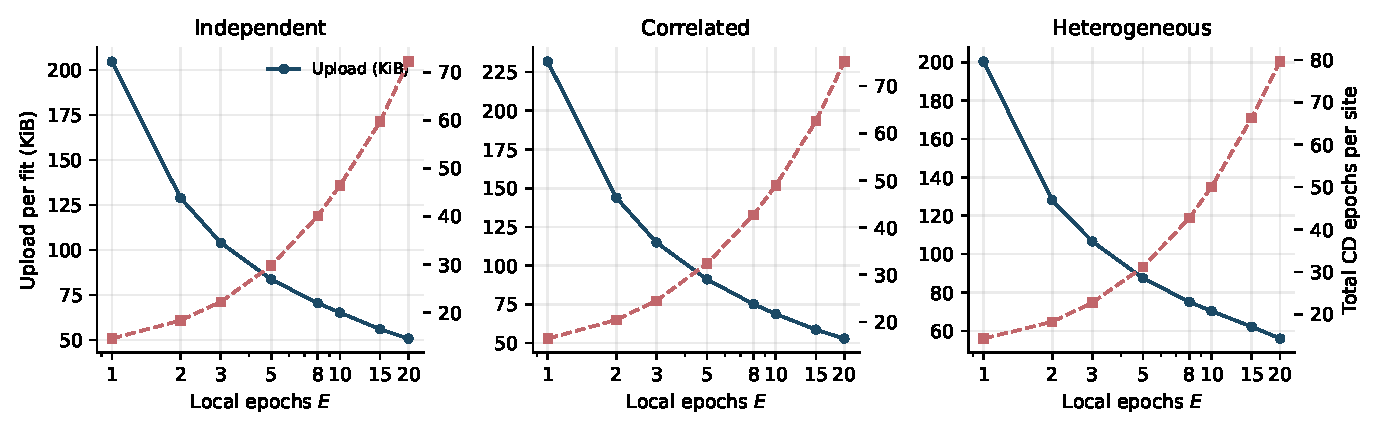
\includegraphics[width=\textwidth]{figures/fig2_cost.pdf}
\caption{The two cost axes for \textsc{FedAvg}. Upload (solid, left axis)
falls in $E$; total coordinate-descent epochs per site (dashed, right axis)
rises. Means over $100$ replicates.}
\label{fig:cost}
\end{figure}

Figure~\ref{fig:cost} makes the accounting point. In the independent
design, moving from $E = 1$ to $E = 20$ cuts rounds from \MIndRoundsOne\ to
\MIndRoundsTwenty\ and upload in proportion, but raises total local work
from \MIndEpochsOne\ to \MIndEpochsTwenty\ coordinate-descent epochs per
site---a factor of five. The correlated and heterogeneous designs behave the
same way (\MCorEpochsOne\ to \MCorEpochsTwenty, and \MHetEpochsOne\ to
\MHetEpochsTwenty). A schedule selected on rounds alone is the schedule
that performs the most arithmetic, and in cross-silo deployments, where
sites are institutions with real compute budgets rather than phones, that
is not obviously the right optimum. Since selection quality is nearly flat
in $E$ once the aggregation is repaired, the choice can be made on cost
alone---which is a more comfortable place to be than choosing $E$ to
protect a variable list.
